

%\hh{lihui: i hid some results to meet 2-page limit (1) check the text/figure/table to see if they are consistent; (2) check if the results here are consistent with what we said in 9-page content (e.g., we say 'xxxx results can be found in appendix there, but here we might have hidden them; (3) why are there two empty pages at the end?}

%\hh{since this part is about reproducibility, we need a short paragraph about datasets/machines/parameters/sourcecode. (1) we can simply say sth like "the description of datasets, machine and parameters can be found in Seciton~xxxx. Both datasets are publicacly available" (2) mention that we will release source code; (3) if we have a video, provide the url here (and in the experimental section) (4) check SYTE kdd submission for some 'standard' language.}

\noindent \textbf{Reproducibility.} Two datasets are used in our experiments, including Yago core version and Covid-19 knowledge graph. All experiments are performed on a machine with an Intel Core-i7 3.00GHz CPU and 64GB memory. The details of datasets, machine and parameters can be found in Section ~\ref{experiment}. All datasets are publicly available. The source code will be released upon publication of the paper. The video demonstration of the system can be found at
\url{https://github.com/lihuiliullh/KompaRe}.


\vspace{-0.3\baselineskip}
\subsection{A -- Predicate Entropy and Similarity Examples}
\vspace{-0.3\baselineskip}
Here, we use Figure ~\ref{inconsistency} to give two examples on how to calculate the predicate entropy and predicate-predicate similarity. 
For the predicate entropy, 
suppose we want to calculate the entropy for {\tt command}. Three entities ({\tt President}, {\tt US Army} and {\tt Air Force}) have {\tt command} as their out links, and the numbers of out links of {\tt command} are 2, 3 and 2, respectively. 
Therefore, 
$V_i^2 = \{{\tt President}, {\tt Air Force} \}$, $V_i^3 = \{ {\tt US Army} \}$ and $V_i^d = \emptyset$ otherwise. Therefore, we have 
$E({\tt command}) = -\frac{2}{3} \log(\frac{2}{3}) - \frac{1}{3}\log(\frac{1}{3}) = 0.92$ and $w({\tt command}) = 0.43$.



\vspace{-0.8\baselineskip}
\subsection{B -- Proof of Lemma ~\ref{lm:collectiveinfluence}}



\vspace{-0.8\baselineskip}
\subsection{C -- Predicate Entropy}

The top-{\em 10} predicates with the highest predicate entropy in Yago dataset are {\tt edited}, {\tt isConnectedTo}, {\tt actedIn}, {\tt playsFor}, {\tt dealsWith}, {\tt directed}, {\tt hasNeighbor}, {\tt isAffiliatedTo}, {\tt wroteMusicFor} and {\tt exports}. Predicates like {\tt actedIn}, {\tt playFor}, {\tt hasNeighbor} have a very high entropy. 
The reason is that these predicates not only occur commonly in the Yago knowledge graph, but also 
have a high degree of uncertainty.
It is consistent with our hypothesis that these predicates provide little semantic information about the entities around them.
On the contrary, The top-{\em 10} predicates with the lowest predicate entropy in Yago dataset are {\tt diedIn}, {\tt hasGender}, {\tt hasCurrency}, {\tt wasBornIn}, {\tt hasAcademicAdvisor},  {\tt isPoliticianOf}, {\tt isMarriedTo}, {\tt hasCaptal}, {\tt hasWebsite}, and {\tt isCitizenOf}. Predicates like {\tt diedIn}, {\tt wasBornIn}, {\tt isMarriedTo}, {\tt isPoliticianOf} have a very low entropy.
They provide specific and detailed background information about the entities around them.

\hide{
\vspace{-0.8\baselineskip}
\subsection{C -- Node-specific Knowledge Segments Results}

Figure ~\ref{nibble-hawaii} shows another node-specific knowledge segment w.r.t. the query node {\tt Hawaii}. We can see 
many landmarks in {\tt Hawaii}, e.g. ,{\tt Hawaii Convention Center}, {\tt Hawaii State Capitol}, {\tt Aloha Stadium}. We also find that {\tt Honolulu} is the capital of {\tt Hawaii}.

\begin{figure}[ht]
\vspace{-0.6\baselineskip}
	\centering
	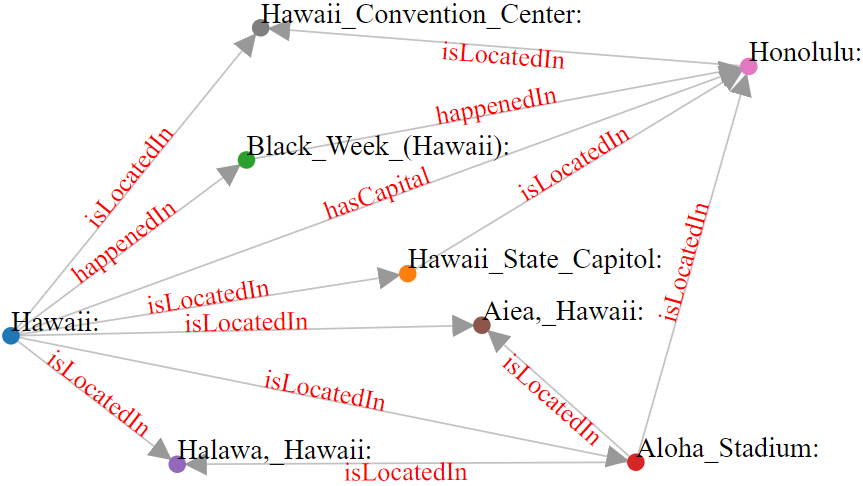
\includegraphics[width=0.35\textwidth, height=0.16\textwidth]{img/nibble-hawaii.png}
	\vspace{-1\baselineskip}
	\caption{Node-specific knowledge segment of {\tt Hawaii}.}
	\label{nibble-hawaii}
	\vspace{-0.8\baselineskip}
\end{figure}
}

{
\vspace{-0.8\baselineskip}
\FloatBarrier
\subsection{D -- Predicate Similarity Results}
Table ~\ref{appendix-pred-sim} shows the predicate similarity between {\tt isTypeOf} and other predicates. %We only list the predicates we used in this paper.
\begin{table}[!htbp]
    \centering
    \vspace{-0.8\baselineskip}
    \scriptsize
    \caption{Predicate similarity of {\tt isTypeOf} with others}
    \vspace{-2\baselineskip}
    \begin{tabular}{ |c|c|c|c|c|c|c|c| }
  \hline
  predicate & sim & predicate & sim & predicate & sim & predicate & sim \\
  \hline
 isCitizenOf &  0.840 &  isLeaderOf &  0.955 & isAffiliatedTo &  0.808 &  isPoliticianOf &  0.917 \\
 livesIn &  0.972 &  owns &  0.945 & exports &  0.706 &  dealsWith &  0.697\\
 hasCapital &  0.786 &  command &  0.216 & happenedIn &  0.767 &  participatedIn &  0.869\\
 worksAt &  0.752 &  isLocatedIn &  0.870 & & & &\\
  \hline
\end{tabular}
\label{appendix-pred-sim}
\end{table}
}
\vspace{-0.8\baselineskip}
\FloatBarrier



